\documentclass{article}
\usepackage{customized_arxiv_ru}

\usepackage[utf8]{inputenc}
\usepackage[english, russian]{babel}
\usepackage[T1]{fontenc}
\usepackage{url}
\usepackage{booktabs}
\usepackage{amsfonts}
\usepackage{nicefrac}
\usepackage{microtype}
\usepackage{lipsum}
\usepackage{graphicx}
\usepackage{natbib}
\usepackage{doi}
\usepackage{amsmath, amsfonts, amssymb, amsthm, mathtools}
\usepackage{algorithm}
\usepackage{algpseudocode}
\theoremstyle{definition}
\newtheorem{definition}{Определение}
\theoremstyle{assumption}
\newtheorem{assumption}{Предположение}
\theoremstyle{lemma}
\newtheorem{lemma}{Лемма}
\theoremstyle{theorem}
\newtheorem{theorem}{Теорема}
\theoremstyle{proposition}
\newtheorem{proposition}{Предложение}


\title{Стохастический метод Ньютона с различным семплингом}
\author{Денис Швейкин
	%% examples of more authors
	\And
	Рустем Исламов
	%% \AND
	%% Coauthor \\
	%% Affiliation \\
	%% Address \\
	%% \texttt{email} \\
	%% \And
	%% Coauthor \\
	%% Affiliation \\
	%% Address \\
	%% \texttt{email} \\
	%% \And
	%% Coauthor \\
	%% Affiliation \\
	%% Address \\
	%% \texttt{email} \\
}
\date{}

\renewcommand{\shorttitle}{Стохастический метод Ньютона с различным семплингом}

%%% Add PDF metadata to help others organize their library
%%% Once the PDF is generated, you can check the metadata with
%%% $ pdfinfo template.pdf
\hypersetup{
	pdftitle={Стохастический метод Ньютона с различным семплингом},
	pdfsubject={},
	pdfauthor={Денис Швейкин, Рустем Исламов},
	pdfkeywords={},
}

\begin{document}
	
	\maketitle
	
	\begin{abstract}
		
		Задача минимизации среднего от большого числа гладких сильно выпуклых функций встречается в машинном обучении повсеместно. Стохастические методы первого порядка, такие как стохастический градиентный спуск (SGD), для этой задачи хорошо изучены. В свою очередь, методы второго порядка, такие как метод Ньютона имеют определенные преимущества, поскольку могут адаптироваться к кривизне задачи. Также они известны своей быстрой сходимостью. Однако стохастические варианты методов типа Ньютон изучены не так хорошо, как методы типа SGD, и имеют ограничения на размеры батчей. Ранее был предложен метод, который не требует таких ограничений. Наша работа исследует этот метод с различными стратегиями семплинга, которые ведут практическим улучшениям.
		
	\end{abstract}
	
	
	\keywords{Стохастический метод Ньютона, стратегии семплинга}
	
	\section{Вступление}
	
	Задача состоит в минимизации функции эмпирического риска, который имеет форму конечной суммы \cite{kovalev2019stochastic}:
	\begin{equation}\label{ERM}
		\underset{x \in \mathbb R^d}{\min} \left[ f(x) \overset{def}{=} \frac{1}{n} \sum \limits_{i=1}^n f_i(x) \right],
	\end{equation}
	где каждая $f_i$ предполагается имеющей липшицев гессиан. 
	
	Как правило, $n$ - общее количество функций - в современных задачах является очень большим числом. Поэтому в виду вычислительное сложности оценки градиента всех $f_i$ на каждом шаге используется стохастический подход. Стохастический градиентный спуск (SGD) \cite{SGD-1} вычисляет градиенты некоторых случайно выбранных $f_i$, что ведет к более вычислительно дешевым итерациям, по сравнению с традиционным градиентным спуском (GD). Метод SGD и его вариации довольно хорошо изучены. Можно отметить следующие плюсы данного метода. Во-первых, теория методов типа SGD не использует ограничений на размер батчей. Поэтому такие алгоритмы могут приниматься даже с малыми размерами батчей. Известно, что простой SGD дает сходимость только к некоторой окрестности оптимума \cite{sgd-hogwild, sgd-general-analysis}. Тем не менее, есть техники (также известные как редукция дисперсии), разрешающие эту проблему. Эти техники \cite{exp-convergence, advances-NIPS, unified-sgd, one-method} модифицируют шаг SGD, что позволяет избавиться от вышеупомянутого эффекта, не меняя вычислительной сложности итерации. Однако главный недостаток всех градиентных методов состоит в том, что вычислительная сложность зависит от кривизны задачи, которая определяется как отношение константы Липшица и параметра сильной выпуклости, и называется числом обусловленности.
	
	Здесь в дело вступают методы второго порядка типа Ньютон \cite{Nesterov-introductory, Newton-convergence, RSN}. Учитывая производные второго порядка, становится возможно адаптировать шаг алгоритма под кривизну задачи \cite{Nesterov-introductory}. К сожалению, намного меньше работы было проведено в направлении стохастических методов типа Ньютон. Многие методы \cite{sub-sampled, exact-inexact, variance-reduced-Newton, zhang2022adaptive, tripuraneni2018stochastic, zhou2020stochastic}. нуждаются в использовании батчей больших размеров. В частности, зачастую необходимый размер батча обратно-квадратично пропорционален желаемой точности. Это значит, что нужно считать гессианы от большого количества $f_i$, которое может иногда даже превышать $n$. \cite{kovalev2019stochastic} предлагает простой стохастический метод Ньютона, который может работать с батчами любого размера. Алгоритм достигает локальной линейной сходимости, а в некоторых случаях - сверхлинейной. 
	
	На практике для алгоритмов типа SGD используются различные стратегии семплинга, улучшающие их качество. Одним из наиболее известных механизмов семплинга является так называемый Importance Sampling (ИС) \cite{gower2019sgd, https://doi.org/10.48550/arxiv.1401.2753, 9413313}. Идея состоит в том, чтобы вычислять градиенты от тех функций, которые вносят наибольший вкладв задачу. Другой метод рандомизированной оптимизации - Random Reshuffling, который делает градиентные шаги, проходясь подряд по случайно перемешанным данным \cite{mishchenko2020random}.
	 \cite{richtarik2016parallel} изучает множество других механизмов семплинга. Мы анализируем эти стратегии, но применительно к Алгоритму 1 из \cite{kovalev2019stochastic}, чтобы получить теоретический и практические улучшения. Мы исследуем различные стратегии семплинга, подкрепляя их строго поставленными экспериментами.
	 
	\section{Постановка задачи}
	
	Мы рассматриваем классическую задачу минимизации функции эмпирического риска (ERM), которая типично возникает во многих задачах машинного обучения в контексте обучения модели. Целевая функция $f$ (\ref{ERM}) является средним от большого количества функций $f_i$, где каждая $f_i$ представляет собой функцию потерь на $i$-том тренировочном объекте. Например, эта нотация может быть применена к линейной регрессии. В данном случае задача состоит в нахождении оптимального вектора параметров $x$, который минимизирует среднеквадратическую ошибку (MSE) на обучающей выборке.
	
	\subsection{Предположения}
	
	Мы делаем стандартные предположения на функции $f_i$; те же, что были приняты в  \cite{kovalev2019stochastic}.
	
	
	\begin{assumption}[Сильная выпуклость] Дифференцируемая функция $\phi:\ \mathbb R^d \rightarrow \mathbb R$ называется $\mu$-сильно выпуклой, где $\mu > 0$, если $\forall\ x, y \in \mathbb R^d$
		
		\begin{equation}\label{strong-conv}
			\phi(x) \geqslant \phi(y) + \langle \nabla \phi, x - y \rangle + \frac{\mu}{2} \| x - y \|^2,
		\end{equation}
	\end{assumption}
	где норма $\| \cdot \|$ - евклидова. Для дважды дифференцируемых функций данное предположение равносильно тому, что все собственные значения гессиана $\geqslant \mu$.
	
	\begin{assumption}[Липшицевы гессианы] Функция $\phi: \mathbb R^d \rightarrow R$ обладает $H$-липшицевым гессианом, если $\forall\ x, y \in \mathbb R^d$
		
		\begin{equation}\label{lip-hess}
			\| \nabla^2 \phi(x) - \nabla^2 \phi(y) \| \leqslant H \| x - y \|
		\end{equation}
	\end{assumption}
	
	\subsection{Семплинг}
	
	\begin{definition}[Семплинг]
		Случайное множественнозначное отображение $\hat S:\ [n] \rightarrow 2^{[n]}$ называется семплингом.
	\end{definition}
	
	Это значит, что каждое $S_k \subseteq [n]$ является реализацией $\hat S$. В таком лсучае мы можем назвать любое вероятностное распределение на $2^{[n]}$ стратегией семплинга.
	
	\subsection{Алгоритм}
	
	Мы применяем различные стратегии семплинга поверх Алгоритма 1 из \cite{kovalev2019stochastic}:
	
	\begin{algorithm}
		\caption{Стохастический метод Ньютона (SN)}\label{SN}
		\begin{algorithmic}
			\item \textbf{Инициализация:} Выбрать начальные приближения $w_1^0, w_2^0, ... w_n^0 \in \mathbb R^d$
			
			\item \For {$k = 0, 1, 2, ...$}	
			
			$ x^{k+1} = \left[ \frac{1}{n} \sum \limits_{i=1}^n \nabla^2 f_i(w_i^k) \right]^{-1} \left[ \frac{1}{n} \sum \limits_{i=1}^n \nabla^2 f_i(w_i^k) w_i^k - \nabla f_i(w_i^k) \right] $
			
			Выбрать подмножество $S^k \subseteq \{ 1, 2, ..., n \}$ одной из стратегий семплинга
			
			$w_i^{k+1} = 
			\begin{cases}
				x^{k+1} & i \in S^k \\
				w_i^k & i \notin S^k
			\end{cases}$
			
			\item \EndFor
		\end{algorithmic}
	\end{algorithm}
	
	\subsection{Цель проекта}
	
	Мы сравниваем различные стратегии семплинга для Алгоритма \ref{SN}, доказывая гарантии сходимости и показывая практические улучшения по сравнению с базовым подходом.
	
	
	\section{Теория}	
	
	\subsection{Доказательство Алгоритма}
	
	Сходимость Алгоритма \ref{SN} была подробно описана и доказана в \cite{kovalev2019stochastic}. Для начала, обратимся к утверждениям трех лемм из данной статьи.
	
	\begin{lemma}\label{lemma:1}
		Пусть $f_i$ - $\mu$-сильна выпукла и имеет $H$-липшицев гессиан для всех $i = 1,...,n$. Рассмотрим следующую функцию Ляпунова
		\begin{equation}
			\mathcal W^k \overset{\text{def}} = \frac{1}{n} \sum \limits_{i=1}^n \| w_i^k - x^* \|^2,
		\end{equation}
		где $x^*$ - точка оптимума для $f$ (\ref{ERM}). Тогда итерации Алгоритма \ref{SN} удовлетворяют
		\begin{equation}
			\|x^{k+1} - x^*\| \leqslant \frac{H}{2 \mu} \mathcal W^k.
		\end{equation}
	\end{lemma}
	
	\begin{lemma}\label{lemma:2}
		Предположим, что каждая $f_i$ - $\mu$-сильно выпукла и имеет $H$-липшицев гессиан. Если $\|w_i^0 - x^*\| \leqslant \frac{\mu}{H}$ для всех $i = 1, ..., n$, тогда для всех $k$
		\begin{equation}
			\mathcal W^k \leqslant \frac{\mu^2}{H^2}.
		\end{equation}
	\end{lemma}
	
	 Последняя лемма - именно та, которая опирается на природу стратегии семплинга. Авторы Алгоритма \ref{SN} используют так называемый $\tau$-nice семплинг, который выбирает подмножество $S^{k} \subseteq \{ 1, 2, ..., n \}$ в точности размера $\tau$ равновероятно. В таком случае можно определить математическое ожидание $\mathbb E_k[\mathcal W^{k+1}] \overset{\text{def}} = \mathbb E[\mathcal W^{k+1} | x^k, w_1^k, ..., w_n^k]$.
	
	\begin{lemma}\label{lemma:3}
		Итерации Алгоритма \ref{SN} с $\tau$-nice семплингом удовлетворяют соотношению
		\begin{equation}
			\mathbb E_k[\mathcal W^{k+1}] = \frac{\tau}{n} \| x^{k+1} - x^* \|^2 + \left(1 - \frac{\tau}{n}\right) \mathcal W^k
		\end{equation}
	\end{lemma}
	
	Далее следует теорема, дающая оценку сходимости Алгоритма \ref{SN} с $\tau$-nice семплингом.
	
	\begin{theorem} \label{theorem:1}
		Предположим, что каждая $f_i$ - $\mu$-сильно выпукла и имеет $H$-липшицев гессиан. Тогда для итераций Алгоритма \ref{SN} выполнено рекуррентное соотношение
		\begin{equation}
			\mathbb E_k[\mathcal W^{k+1}] \leqslant \left( 1 - \frac{\tau}{n} + \frac{\tau}{n} \left( \frac{H}{2\mu} \right)^2 \mathcal W^k \right) \mathcal W^k.
		\end{equation}
		Кроме того, если $\forall i\ \|w_i^0 - x^*\| \leqslant \frac{\mu}{H}$, то
		\begin{equation}
			\mathbb E_k[\mathcal W^{k+1}] \leqslant \left( 1 - \frac{3\tau}{4n} \right) \mathcal W^k.
		\end{equation}
	\end{theorem}
	
	
	\subsection{Стратегии семплинга}
	
	\subsubsection{Вдвойне однородные сратегии}
	
	Для начала рассмотрим стратегии семплинга, представленные в \cite{richtarik2016parallel} в отношении покоординатных методов. Эти стратегии являются \textit{вдвойне однородными.}
	
	\begin{definition}[Вдвойне однородный (Doubly Uniform, DU) семплинг] \label{DU}
		Это такие стратегии, которые возвращают все множества одинаковой мощности с одинаковой вероятностью. То есть если $|S_1| = |S_2|$, то $\mathbb P(S_1) = \mathbb P(S_2)$.
	\end{definition}
	
	Название обусловлено тем, что данное свойство сильнее, чем \textit{однородность}, которая означает, что все $i \in [n]$ имеют одинаковую вероятность быть включенными в выбранное множество $\hat S$. Это можно увидеть, если обозначить вероятность $q_j = \mathbb P(|\hat S| = j)$ для всех $j = 0, 1, ... n$. Тогда для всех $S \subseteq [n]$ имеем $\mathbb P(S) = q_j / \binom{n}{j}$. Отсюда
	\begin{equation}
		p_i = \sum \limits_{j=1}^n \sum \limits_{|S|=j, i \in S} \mathbb P(S) = \sum \limits_{j=1}^n \sum \limits_{|S|=j, i \in S} \frac{q_j}{\binom{n}{j}} = \sum \limits_{j=1}^n   \frac{\binom{n-1}{j-1}q_j}{\binom{n}{j}} = \frac{1}{n} \sum \limits_{j=1}^n j q_j = \frac{\mathbb E[|\hat S|]}{n}
	\end{equation}
	
	Ясно, что вдвойне однородная стратегия семплинга задается вектором $q$ распределения вероятностей на всевозможных размерах $j = 0, 1, ..., n$ множества $\hat S$. Представляют интерес несколько DU-стратегий.
	
	\begin{enumerate}
		\item \textbf{$\tau$-nice семплинг.}\label{nice} Зафиксируем $1 \leqslant \tau \leqslant n$. Семплинг называется $\tau$-nice, если он является DU с $q_\tau = 1$. Именно эта стратегия используется авторами Алгоритма \ref{SN}. Эту стратегию можно интерпретировать в терминах параллельных вычислений. Так, пусть есть $\tau$ доступных процессоров. В момент семплинга мы выбираем батч размера $\tau$ и назначаем каждый объект $i \in \hat S$ одному процессору. Таким образом, каждый процессор обновит значение целевой функции, градиенты и гессианы в соответствии с новым $w_i^k$.
		
		\item \textbf{$\tau$-независимый семплинг.}\label{tau-ind} Зафиксируем $1 \leqslant \tau \leqslant n$. $\tau$-независимым семплингом называется DU-семплинг с
		\begin{equation} 
			q_k = 
			\begin{cases}
				\binom{n}{k}c_k, & k = 1, 2, ..., \tau \\
				0, & k = \tau + 1, ..., n
			\end{cases}
		\end{equation}
		где $c_1 = (1/n)^\tau$ и $c_k = (k/n)^\tau - \sum \limits_{i=1}^{k-1} \binom{k}{i}c_i$ for $k \geqslant 2$.
		
		Интерпретация состоит в том, что каждый из $\tau$ процессоров выбирает один из объектов обучающей выборки $i \in [n]$. Если несколько процессоров выбрали один и тот же объект, то только один из них получает доступ к нему. Эта стратегия легко реализуема в терминах параллельных вычислений. Кроме того, если батчи невелики, мы имеем $\tau \ll n$, и тогда $\tau$-независимый семплинг хорошо приближает $\tau$-nice.
		
		\item \textbf{$(\tau, p_b)$-биномиальный семплинг.}\label{tau-bin} Фиксируем $1 \leqslant \tau \leqslant n$ и $0 \leqslant p_b \leqslant 1$. Стратегия является DU-семплингом с
		\begin{equation}
			q_k = \binom{\tau}{k}p_b^k(1 - p_b)^k, \quad k \leqslant \tau
		\end{equation}
		Это модель ситуации, когда каждый из $\tau$ процессоров доступен в момент семплинга с вероятностью $p_b$, отсюда $q_k$ - вероятность того, что $k$ процессоров оказались доступны.
	\end{enumerate}
	
	\subsubsection{Независимые стратегии}
	
	Кроме вдвойне однородных стратегий, мы рассматриваем такие стратегии, которые принимают решение о каждом тренировочном объекте $i \in [n]$ независимо, со своей вероятностью $p_i$. Отметим, что в случае $p_1 = p_2 =...= p_n$ стратегия остается DU. Однако в общем случае появляются некоторые изменения в оценке скорости сходимости. Существует стратегия, называемая \textit{importance sampling}, которая присваивает вероятности пропорционально константам Липшица (\ref{lip-hess}) гессианов $\nabla^2 f_i(x)$ (или градиентов $\nabla f_i(x)$).
	
	\textbf{Importance sampling (ИС).}\label{imp-hess} Стратегия задает вероятности
	\begin{equation}
		p_i = \frac{H_i}{\sum \limits_{i=1}^n H_i}
	\end{equation}
	
	\subsubsection{Последовательная стратегия}
	
	Наконец, мы изучаем стратегию, состоящую в последовательном проходе по перемешанным данным:
	
	\textbf{Последовательная стратегия.}\label{consec} На первой итерации Алгоритма \ref{SN} фиксируется случайная перестановка $\pi$ обучающей выборки $[n]$ и размер батча $\tau$. Далее на итерации номер $k$ берутся объекты с номерами:
	\begin{equation}
		\pi(k+1\ \text{mod}\ n), \pi(k+2\ \text{mod}\ n), ..., \pi(k+\tau\ \text{mod}\ n).
	\end{equation}
	А если $(k\ \text{mod}\ n) + \tau > n$, то берутся все объекты с номерами между $k\ \text{mod}\ n$ и $n$, то есть на данном шаге размер батча может быть меньше $\tau$.
	
	\subsection {Скорость сходимости}
	
	\subsubsection{Оценки для вдвойне однородного семплинга}
	
	Чтобы установить скорость сходимости Алгоритма \ref{SN} с вдвойне однородным семплингом (\ref{DU}), обратимся к Лемма \ref{lemma:3}, поскольку это первое место в доказательстве Алгоритма \ref{SN}, которое зависит от стратегии семплинга. Она обобщается на произвольный DU-семлпинг.
	
	\begin{lemma} \label{lemma:4}
		Итерации Алгоритма \ref{SN} с вдвойне однородным семплингом удовлетворяют
		\begin{equation}
			\mathbb E_k[\mathcal W^{k+1}] = p \mathbb E_k[\| x^{k+1} - x^* \|^2] + \left(1 - p \right) \mathcal W^k,
		\end{equation}
		где $p = \frac{\mathbb E[|\hat S|]}{n}$.
	\end{lemma}
	\begin{proof}
		Свойство вдвойне однородности влечет, что все объекты имеют одинаковую вероятность $p = \frac{\mathbb E[|\hat S|]}{n}$ быть включенными в выбранное множество $\hat S$. Таким образом, в силу линейности математического ожидания, получаем требуемое.
	\end{proof}
	Тогда итоговая оценка имеет ту же форму, что и представлено в \cite{kovalev2019stochastic}:
	\begin{equation}\label{DU convergence}
		\mathbb E_k[\mathcal W^{k+1}] \leqslant \left( 1 - p + p \left( \frac{H}{2\mu} \right)^2 \mathcal W^k \right) \mathcal W^k
	\end{equation}
	в общем случае, а для $\forall i\ \| w_i^0 - x^* \| \leqslant \frac{\mu}{H}$:
	\begin{equation}
		\mathbb E_k[\mathcal W^{k+1}] \leqslant \left( 1 - \frac{3}{4}p \right) \mathcal W^k.
	\end{equation}
	
	Значит, если зафиксировать ожидаемый размер батча $\mathbb E [|\hat S|] = \tau$, то скорость сходимости такая же, как и у $\tau$-nice семплинга.
	
	\subsubsection{Независимые и последовательная стратегии}
	
	Теперь рассмотрим общий случай выбора каждого объекта независимо с вероятностью $p_i$.
	
	\begin{proposition} \label{proposition:1}
		На каждой конкретной итерации Алгоритма \ref{SN} при фиксированном матожидании размера батча $\mathbb E_k[|\hat S^k|] = \tau$ минимальное значение в оценке $\mathbb E_k[\mathcal W^{k+1}]$ достигается, если задать $p_i = 1$ для некоторых $i \in [n]$, возможно $p_i \in (0, 1)$ для одного $i$, и $p_i = 0$ для остальных.
	\end{proposition}
	
	\begin{proof}
		Мы можем обобщить оценку из Леммы \ref{lemma:4} на наш случай.
		\begin{equation}
			n \cdot \mathbb E_k[\mathcal W^{k+1}] = \sum \limits_{i=1}^n p_i  \| x^{k+1} - x^* \|^2 + \sum \limits_{i=1}^n \left(1 - p_i \right) \|w_i^k - x^*\|^2.
		\end{equation}
		Учитывая $\tau = \mathbb E_k[|\hat S^k|] = \sum \limits_{i=1}^n p_i$, имеем
		\begin{equation}
			n \cdot \mathbb E_k[\mathcal W^{k+1}] = \left( \tau  \| x^{k+1} - x^* \|^2 + n \cdot \mathcal W^k \right) - \sum \limits_{i=1}^n p_i \|w_i^k - x^*\|^2.
		\end{equation}
		То есть задача состоит в максимизации $\sum \limits_{i=1}^n p_i \|w_i^k - x^*\|^2$ при следующем условии:
		\begin{equation} \label{polyhedron}
			\begin{cases}
				\sum \limits_{i=1}^n p_i = \tau \\
				0 \leqslant p_i \leqslant 1\ \forall i
			\end{cases}
		\end{equation}
		Решением данной задачи линейного программирования является вершина многогранника, задаваемого ограничениями (\ref{polyhedron}). Оптимальная вершина имеет максимальную проекцию своего координатного вектора $(p_1, ..., p_n)^\top$ на вектор $(\|w_i - x^*\|^2, ..., \|w_n - x^*\|^2)$. Это та вершина, коэффициенты которой, отвечающие наибольшим $\|w_i - x^*\|^2$ установлены равными 1, отвечающие наименьшим $\|w_i - x^*\|^2$ установлены равными 0, и одна координата имеет промежуточное значение, если $\tau$ не целое.
	\end{proof}
	
	В таком случае мы видим, что имеет смысл обновлять те векторы параметров $w_i^k$, которые не обновлялись дольше других. Это значит, что оптимальная независимая стратегия может быть "приближена" последовательной стратегией. Данное предложение иллюстрируется в секции экспериментов (\ref{fig:3}).
	
	
	\subsubsection{Замечания о Importance Sampling}
	
	В некоторых методах, в частности, в традиционном SGD, преимущество применения ИС состоит в том, чтобы заменить оценки, основанные на $H_{max}$ - максимуме из констант Липшица $H_i$ каждой $f_i$ - оценками, обусловленными $\overline H$ - среднему значению всех $H_i$. Данное улучшение достигается благодаря рассмотрению задачи, похожей на оригинальную (\ref{ERM}), но где каждая $f_i$ масштабирована обратно пропорционально $H_i$ для того, чтобы сохранить математическое ожидание  $f(x)$ и $\nabla f(x)$ равными истинным значениям $f$ и $\nabla f(x)$.
	
	Однако Алгоритм \ref{SN} имеет немного другую природу. Это значит, что направление шага оценивается по информации не только лишь от тех объектов, которые включены в батч на текущей итерации. Оно вычисляется, учитывая всю информацию с предыдущего шага, с небольшими изменениями на текущем шаге. Следовательно, вышеупомянутая техника не может быть применена напрямую. В таком случае оказывается очень трудно установить какие-либо конкретные оценки для ИС применительно к Алгоритму \ref{SN}.
	
	\section{Эксперименты}
	
	Мы проводим эксперименты на данных, полученных с помощью функции {\fontfamily{qcr}\selectfont make\_classification} из библиотеки {\fontfamily{qcr}\selectfont sklearn} с 500 объектами и 5 признаками. Код эксперимента доступен в репозитории проекта (\href{https://github.com/intsystems/2023-Project-136/tree/master/code}{ссылка}). Оптимизируем логистическую функцию с $l_2$-регуляризацией: $f_i(x) = \log(1 + \exp(-b_i \cdot a_i^T x)) + \frac{\lambda}{2}\|x\|_2^2$, где $x, a_1, ..., a_n \in \mathbb R^d$, $b_i = \pm 1$ и константа регуляризации $\lambda$ равна 0.01. На каждой картинке представлено два графика. Первый отражает траекторию величины $\mathcal W^k = \frac{1}{n} \sum \limits_{i=1}^n \|w_i^k - x^* \|^2$, а второй - историю невязки по функции. Ось $x$ - количество полных проходов по датасету. 
	
	\subsection{Вдвойне однородные стратегии}
	\begin{figure}[h!]\label{fig:1}
		\centering
		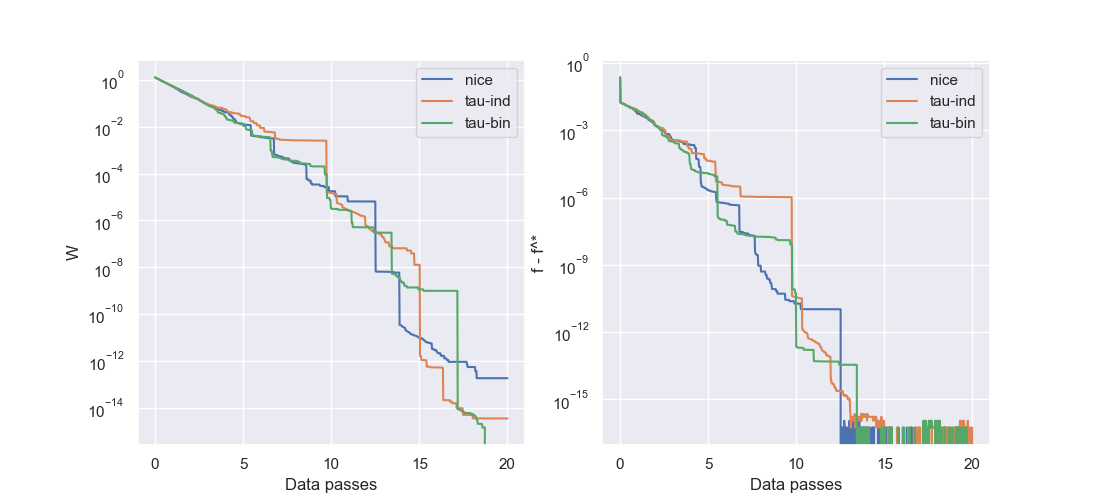
\includegraphics[width=\textwidth]{uniform strategies}
		\caption{Сравнение стратегий $\tau$-nice, $\tau$-независимой и $\tau$-биномиальной}
	\end{figure}
	Мы видим, что все вдвойне однородные стратегии с одинаковым математическим ожиданием размера батча демонстрируют одинаковую скорость сходимости.
	
	\subsection{Importance Sampling}
	\begin{figure}[h!]\label{fig:2}
		\centering
		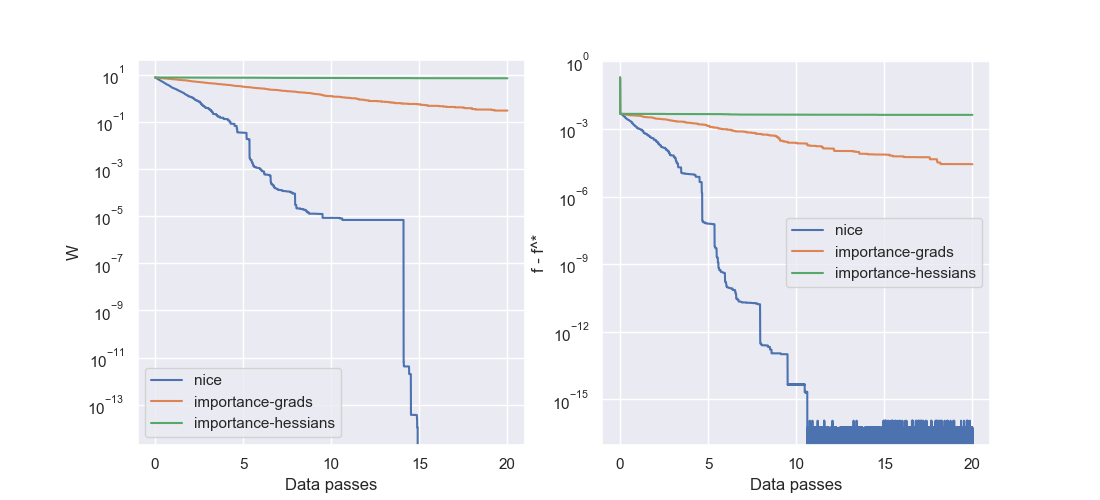
\includegraphics[width=\textwidth]{importance sampling}
		\caption{Сравнение $\tau$-nice семплинга и Importance Sampling}
	\end{figure}
	Мы применяем ИС, основанный как на липшицевости гессианов, так и градиентов. Для задачи логистической регрессии константы Липшица равны $H_i = \frac{1}{10} \|a_i\|^3$ и $L_i = \frac{1}{4}\|a_i\|^2$ соответственно. Видно, что для рассматриваемой задачи ИС, примененный к Алгоритму \ref{SN}, не дает практических улучшений.
	
	\subsection{Последовательная стратегия}
	\begin{figure}[h!]\label{fig:3}
		\centering
		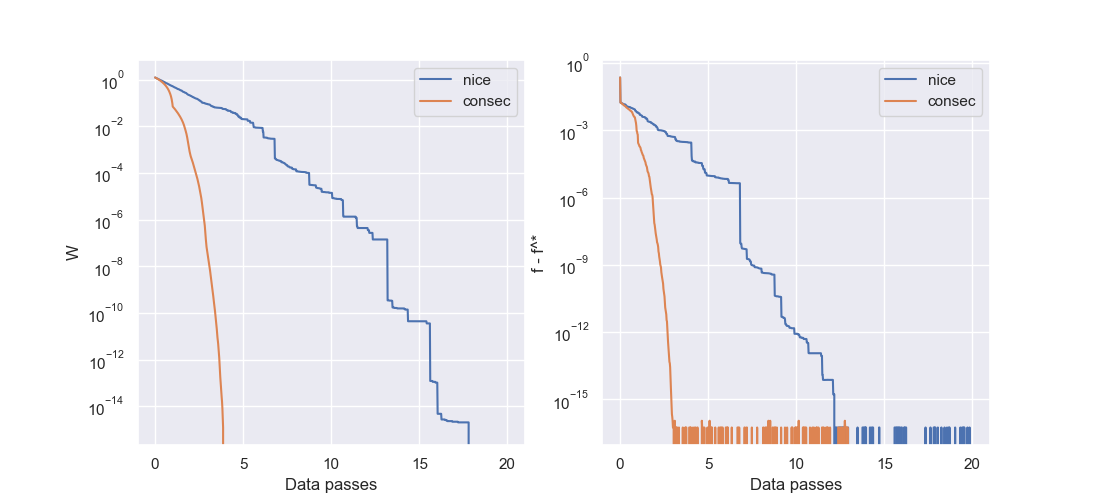
\includegraphics[width=\textwidth]{consecutive strategy 10}
		\caption{Сравнение $\tau$-nice и последовательной стратегии}
	\end{figure}
	В данном случае имеется практическое улучшение. Последовательная стратегия превосходит базовую $\tau$-nice. Тем не менее, теоретическое обоснование этого факта остается неясным.
	
	\section{Заключение}
	Таким образом, мы приводим сравнение различных стратегий семплинга, применяемых к Стохастическому методу Ньютона (\ref{SN}). Во-первых, мы обощаем линейную оценку скорости сходимости на все вдвойне однородные стратегии и устанавливаем практическую эквивалентность наиболее популярных представителей данного класса (Лемма \ref{lemma:4}, Уравнение \ref{DU convergence}, Рис. \ref{fig:1}). Во вторых, мы получаем, что Importance Sampling маловероятно будет превосходить стандартную стратегию $\tau$-nice, а на практике сильно уступает (Рис. \ref{fig:2}). Наконец, улучшения появляются при использовании последовательной стратегии (Рис. \ref{fig:3}). Это, безусловно, положительный эффект, и он требует дальнейшего изучения.
	
	
	% references title
	\renewcommand\refname{References}	
	\bibliographystyle{plain}
	\bibliography{references}
	
\end{document}
